\section{Graphical Design}
\label{sec:graphical_design}

Based on our analysis, we concluded that there does not seem to be a relation between the complexity of the graphics, and the impact this has on how much fun or educating a game is.
For this reason 2D graphics has been deemed appropriate for this game.
The following section will go through the design choices that have been made in terms of the different graphical interfaces of the game, along with justification for why a given choice was made. The graphical interfaces includes the board, the editor and the menu.

\subsection{Board}
The board is a hexagon consisting of hexagonal tiles.
This means that by design the entire field is hexagons in hexagons. 
A cell takes up a single tile on the board, as does the various food types a player may encounter.
Hexagons were chosen for the map, because they add further complexity to the game in terms of 'legal movements' for a cell, relative to if we had chosen squares, see \autoref{sec:designing_playing_field}.
Hexagons seemed a good design choice, it adds the structure we need as programmers, and it opens up more avenues of play for the players.
A mock-up of the board can be seen on \autoref{fig:cells_mockup}.\newline

\begin{figure}[ht]
	\centering
		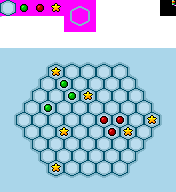
\includegraphics{img/cells_mockup.png}
	\caption{Playing field with cells and food}
	\label{fig:cells_mockup}
\end{figure}

Food in this example is a star.
We have created other mock-ups as well, such as a ham and an egg as possible alternatives. 
Cells are illustrated on the map in green and red, with green referring to one player's cells, and red referring to another player's cells.
The icons chosen for cells and food have been chosen for the sole purpose of added clarity, that a player can within reason quickly distinct between food and their cells, and their opponent's cells.
Choosing different colours for cells is an easy was to achieve this distinction.
With all food types taking a none-circular shape or a totally different color-scheme, such as a yellow star, it will also help the players distinct between what is food and what are actual player controlled entities.

\subsection{Health Bar}
It was decided to design a health bar at the top of the board to give the player an indication of how well they are doing in the game, shown on \autoref{fig:healthbar}.
The idea is that the health bar will fill with green and red colors, depending on the current of all cells on the player's team.
If the bar is completely green, the player has won the game, and likewise they will lose the game, if the bar fills with red.
The amount of red and green color is determined entirely by the total amount of energy that the players cells have in contrast to the amount of total energy the enemy cells have.
The basic idea is, that the bar will update throughout the game, sweeping back and forth depending on which player is doing best at the time.
\autoref{fig:healthbar} illustrates how it would look like if the green player has an advantage over the red player during the game.

\begin{figure}[ht]
	\centering
		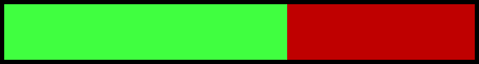
\includegraphics{img/healthbar_example.png}
	\caption{Health bar, where the player has an advantage over his opponent}
	\label{fig:healthbar}
\end{figure}

\subsection{Menu Design}
The menu should somehow resemble the design choices that were made for the board, to make the look of the game consistent.
Therefore, we have worked on a hexagonal design for the background behind each button.\newline

\begin{figure}[ht]
	\centering
		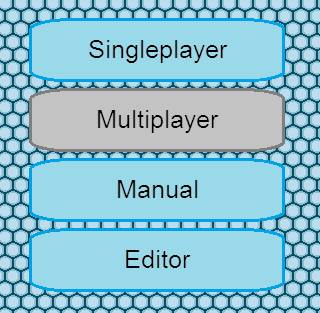
\includegraphics{img/final_menu.png}
	\caption{First menu screen the user sees}
	\label{fig:menu1}
\end{figure}

The color scheme is the same as the board, which is a mixture of light and darker blue colour. 
Options, that are not available to the user, e.g because the user has to unlock them by completing challenges, will be drawn in a grey color scheme to symbolize inactivity.
Greying out inaccessible parts of the program seems highly used in other types of software, such as Windows and various video games, so the same convention will be used for this game.
Accessible options of the menu will be colored in a more vibrant, light blue, to distinct them from the gray buttons.\newline


When a user clicks a menu button, a new menu will be produced.
The menu will represent potential options for the user to take, and they will follow the same color scheme as described previously.